\documentclass[11pt]{article}

\usepackage[T1]{fontenc}
\usepackage[utf8]{inputenc}
\usepackage[french]{babel}
\usepackage{amsmath, amssymb, amsthm}
\usepackage{graphicx}
\usepackage{geometry}
\usepackage{enumitem}
\usepackage{hyperref}
\usepackage{mdframed}
\usepackage{mathtools}

\geometry{margin=2.5cm}

% --- Macros utiles ---
\newcommand{\RR}{\mathbb{R}}
\newcommand{\NN}{\mathbb{N}}
\newcommand{\oo}{+\infty}
\newcommand{\fonction}[5]{#1 : #2 \to #3,\quad #4 \mapsto #5}
\newcommand{\acompleter}{\fbox{À compléter}}

% --- Style des cadres ---
\mdfdefinestyle{coursbox}{
  linewidth=0.8pt,
  linecolor=black,
  backgroundcolor=white,
  roundcorner=0pt,
  innertopmargin=8pt,
  innerbottommargin=8pt,
  innerleftmargin=10pt,
  innerrightmargin=10pt,
  skipabove=10pt,
  skipbelow=10pt
}

% --- Environnements simples ---
\newenvironment{remarque}{\par\smallskip\noindent\textbf{Remarque. \\}\ignorespaces}{\par\smallskip}
\newenvironment{remarques}{\par\smallskip\noindent\textbf{Remarques. \\}\ignorespaces}{\par\smallskip}
\newenvironment{exemple}{\par\smallskip\noindent\textbf{Exemple. \\}\ignorespaces}{\par\smallskip}
\newenvironment{exemples}{\par\smallskip\noindent\textbf{Exemples. \\}\ignorespaces}{\par\smallskip}
\newenvironment{demonstration}{\par\smallskip\noindent\textbf{Démonstration. \\}\ignorespaces}{\par\smallskip}

% --- Environnements encadrés ---
\newmdenv[style=coursbox]{definition}
\newmdenv[style=coursbox]{propriete}

\begin{document}

\begin{definition}
\begin{center}
    {\Huge\bfseries Suites numériques - 1/2}
\end{center}
\end{definition}

\begin{remarque}
Dès l'Antiquité, Archimède de Syracuse (287--212 av. J.-C.) met en œuvre une procédure itérative pour trouver une approximation du nombre $\pi$. Il encadre le cercle par des polygones inscrits et circonscrits ayant un nombre de côtés de plus en plus grand. Par ce procédé, Archimède donne naissance, sans le savoir, à la notion de suite numérique.

Vers la fin du XVII\textsuperscript{e} siècle, des méthodes semblables sont utilisées pour résoudre des équations de façon approchée dans des problèmes de longueurs, d'aires ou de volumes.

Un formalisme plus rigoureux de la notion de suite n'apparaît qu'au début du XIX\textsuperscript{e} siècle avec le mathématicien français Augustin-Louis Cauchy (1789--1857), qui développe une théorie de la convergence et établit les bases de l'analyse des suites numériques.
\end{remarque}

\section{Définition et notations}

\begin{definition}
Une \emph{suite numérique} est une fonction définie sur tout ou partie de l'ensemble $\NN$ des nombres entiers naturels, à valeurs dans $\RR$.
\end{definition}

\begin{remarques}
\begin{itemize}
    \item L'image d'un entier naturel $n$ par la suite $u$ peut se noter $u(n)$ ou, plus simplement, $u_n$ (notation indicielle).
    \item $u_n$ est le \emph{terme général}, ou le \emph{terme d'indice} $n$, ou le \emph{terme de rang} $n$ de la suite.
    \item La suite elle-même se note $u$, $(u_n)$ ou $(u_n)_{n\in\NN}$.
\end{itemize}
\end{remarques}

\begin{exemples}
\begin{itemize}
    \item Soit la suite
    \[
    \fonction{u}{\NN}{\RR}{n}{2n}.
    \]
    $u$ est la suite de terme général $u_n=2n$. On a $u_0=0$, $u_1=2$, $u_2=4$, $u_3=6$, etc. C'est la suite des nombres pairs.

    \item Soit la suite
    \[
    \fonction{v}{\NN}{\RR}{n}{n^2}.
    \]
    $v$ est la suite de terme général $v_n=n^2$. On a $v_0=0$, $v_1=1$, $v_2=4$, $v_3=9$, etc. C'est la suite des carrés parfaits.
\end{itemize}
\end{exemples}

\section{Génération d'une suite}

On définit une suite en indiquant une formule ou un procédé permettant de générer n'importe lequel de ses termes. On utilise deux modes de définition.

\subsection{Définition explicite}

\begin{definition}
Une suite est définie de façon \emph{explicite} lorsque chaque terme s'exprime en fonction de son rang, c'est-à-dire lorsqu'on a une relation du type $u_n=f(n)$ pour une certaine fonction $f$.
\end{definition}

\begin{exemple}
La suite des carrés parfaits est définie pour $n\geq0$ par $u_n=n^2$.

Le calcul des termes est direct. Par exemple, pour le terme de rang $100$ :
\[
u_{100}=100^2=10\,000.
\]
\end{exemple}

\subsection{Définition par récurrence}

\begin{definition}
Une suite est définie \emph{par récurrence} lorsque chaque terme est exprimé en fonction d'un ou de plusieurs termes précédents et que l'on connaît l'un des termes (très souvent le terme initial).
\end{definition}

\begin{remarque}
Pour ce type de suite, le calcul d'un terme ne peut se faire qu'après le calcul du ou des termes précédents.
\end{remarque}

\begin{exemple}
Soit $u$ la suite définie pour $n\geq0$ par
\[
u_0=0,\qquad u_{n+1}=2u_n+1.
\]
Calculer $u_6$.

Pour calculer $u_6$, il faut connaître $u_5$, donc $u_4$, $u_3$, etc. On calcule successivement :
\begin{align*}
u_1&=2u_0+1=2\times0+1=1,\\
u_2&=2u_1+1=2\times1+1=3,\\
u_3&=2u_2+1=7,\\
u_4&=2u_3+1=15,\\
u_5&=2u_4+1=31,\\
u_6&=2u_5+1=63.
\end{align*}
\end{exemple}

\section{Représentations graphiques d'une suite}

Dans un repère $(O\,;\,\vec{i}\,;\,\vec{j})$ du plan, la représentation graphique de la suite $u$ de terme général $u_n$ est l'ensemble des points de coordonnées $(n\,;\,u_n)$ pour $n\in\NN$.

\begin{exemple}
\begin{center}
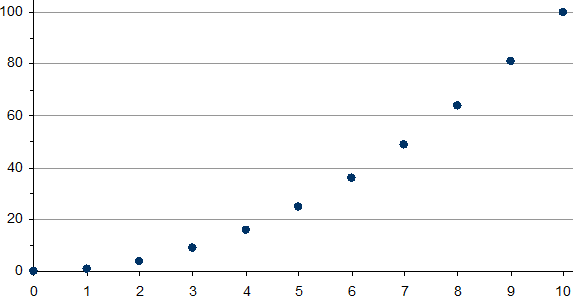
\includegraphics[width=0.6\textwidth]{images/Graphe_carres_parfaits.png}

\emph{Représentation graphique des premiers termes de la suite des carrés parfaits}
\end{center}
\end{exemple}

On peut également placer les nombres $u_0$, $u_1$, $u_2$, etc., sur la droite des réels.

\begin{exemple}
\begin{center}
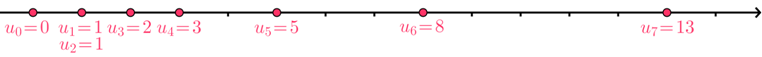
\includegraphics[width=0.7\textwidth]{images/Droite_suite_Fibonacci.png}

\emph{Représentation graphique des premiers termes de la suite de Fibonacci}
\end{center}
\end{exemple}

\section{Sens de variation d'une suite}

\subsection{Définitions}

\begin{definition}
\begin{itemize}
    \item Une suite est dite \emph{croissante} lorsque chaque terme est supérieur ou égal au précédent, c'est-à-dire lorsque, pour tout $n\in\NN$, $u_n\leq u_{n+1}$, ou encore $u_{n+1}-u_n\geq0$.
    \item Une suite est dite \emph{décroissante} lorsque chaque terme est inférieur ou égal au précédent, c'est-à-dire lorsque, pour tout $n\in\NN$, $u_n\geq u_{n+1}$, ou encore $u_{n+1}-u_n\leq0$.
    \item Une suite dont tous les termes sont égaux est dite \emph{constante}.
\end{itemize}
\end{definition}

\begin{exemples}
\begin{itemize}
    \item La suite des nombres pairs et la suite des carrés parfaits sont croissantes.
    \item Soit $u$ la suite définie pour $n\geq1$ par $u_n=\dfrac{1}{n}$. Pour tout entier $n\geq1$,
    \[
    \frac{1}{n}\geq\frac{1}{n+1},
    \]
    donc $u$ est décroissante.
    \item La suite de Syracuse du nombre $17$ n'est ni croissante ni décroissante.
\end{itemize}
\end{exemples}

\begin{remarque}
Une suite n'a pas forcément le même sens de variation sur tout $\NN$ : elle peut être croissante, décroissante ou constante par intervalles.
\end{remarque}

\begin{exemples}
\begin{enumerate}[label=\arabic*.]
    \item Soit la suite $(u_n)_{n\in\NN}$ définie par $u_n=n^2-4n+4$. Démontrer que la suite $u$ est croissante à partir d'un certain rang.
    \item Soit la suite $(v_n)_{n\in\NN^*}$ définie par $v_n=\dfrac{1}{n(n+1)}$. Démontrer que la suite $v$ est décroissante.
\end{enumerate}

\begin{enumerate}[label=\arabic*.]
    \item On calcule la différence $u_{n+1}-u_n$ :
    \begin{align*}
    u_{n+1}-u_n
    &=(n+1)^2-4(n+1)+4-(n^2-4n+4)\\
    &=n^2+2n+1-4n-4+4-n^2+4n-4\\
    &=2n-3.
    \end{align*}
    On a $u_{n+1}-u_n\geq0$ lorsque $2n-3\geq0$, c'est-à-dire pour $n\geq1{,}5$. Comme $n$ est entier, pour tout $n\geq2$, $u_{n+1}-u_n\geq0$. La suite $u$ est donc croissante à partir du rang $2$.

    \item On calcule le rapport :
    \[
    \frac{v_{n+1}}{v_n}
    =\frac{\dfrac{1}{(n+1)(n+2)}}{\dfrac{1}{n(n+1)}}
    =\frac{n}{n+2}.
    \]
    Comme $n<n+2$, on a $\dfrac{v_{n+1}}{v_n}<1$. Or $v_n>0$, donc $v_{n+1}<v_n$. La suite $v$ est décroissante pour tout $n\in\NN^*$.
\end{enumerate}
\end{exemples}

\subsection{Variations d'une suite définie par une fonction}

\begin{propriete}
Soit $f$ une fonction définie sur $\RR^+$ et $(u_n)$ une suite numérique définie sur $\NN$ par $u_n=f(n)$. Soient $a$ et $b$ deux entiers naturels tels que $a<b$.
\begin{itemize}
    \item Si $f$ est croissante sur l'intervalle $[a\,;b]$, alors la suite $(u_n)$ est croissante sur $[a\,;b]$.
    \item Si $f$ est décroissante sur l'intervalle $[a\,;b]$, alors la suite $(u_n)$ est décroissante sur $[a\,;b]$.
\end{itemize}
\end{propriete}

\begin{remarque}
La réciproque est fausse. La représentation ci-dessous montre une suite décroissante alors que la fonction $f$ correspondante n'est pas décroissante.
\begin{center}
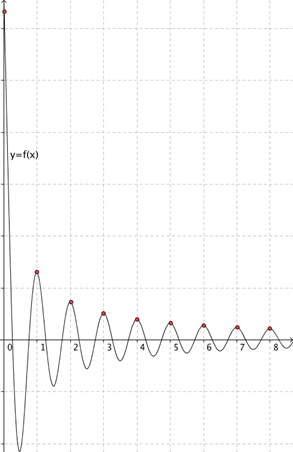
\includegraphics[width=0.6\textwidth]{images/suites_1.png}
\end{center}
\end{remarque}

\begin{exemple}
Pour tout $n\in\NN$, on donne la suite $(u_n)$ définie par $u_n=\dfrac{1}{n+1}$. Démontrer que la suite $(u_n)$ est décroissante.

On considère la fonction associée
\[
\fonction{f}{\RR^+}{\RR}{x}{\frac{1}{x+1}}.
\]
Ainsi, $u_n=f(n)$. Pour tout $x\in\RR^+$,
\[
f'(x)=-\frac{1}{(x+1)^2}<0.
\]
La fonction $f$ est donc décroissante sur $[0\,;+\infty[$. On en déduit que la suite $(u_n)$ est décroissante.
\end{exemple}

\section{Notion de limite d'une suite}

\subsection{Suite convergente}

\begin{definition}
Si, lorsque $n$ devient grand, les termes $u_n$ se rapprochent autant que l'on veut d'un nombre réel $\ell$, on dit que la suite \emph{converge} vers $\ell$, ou encore que la suite a pour \emph{limite} $\ell$.

On note
\[
\lim_{n\to+\infty}u_n=\ell.
\]
\end{definition}

\begin{exemple}
Soit la suite $(u_n)_{n\in\NN^*}$ définie par $u_n=\dfrac{2n+1}{n}$.

On construit le tableau de valeurs suivant :
\[
\begin{array}{c|ccccccccc}
n & 1 & 2 & 3 & 4 & 5 & 10 & 15 & 50 & 500\\ \hline
u_n & 3 & 2{,}5 & 2{,}333 & 2{,}25 & 2{,}2 & 2{,}1 & 2{,}067 & 2{,}02 & 2{,}002
\end{array}
\]
Plus $n$ devient grand, plus les termes de la suite semblent se rapprocher de $2$. On dit que la suite $(u_n)$ converge vers $2$ et on note
\[
\lim_{n\to+\infty}u_n=2.
\]
\end{exemple}

\subsection{Suite divergente}

\begin{definition}
Une suite qui n'est pas convergente est \emph{divergente}. Soit elle n'a pas de limite, soit sa limite est $+\infty$ ou $-\infty$.
\end{definition}

\begin{exemples}
Conjecturer la divergence des suites suivantes :
\begin{enumerate}[label=\arabic*.]
    \item $(u_n)_{n\in\NN}$ définie par $u_n=n^2+1$ ;
    \item $(v_n)_{n\in\NN}$ définie par
    \[
    v_{n+1}=(-1)^n v_n,\qquad v_0=2.
    \]
\end{enumerate}

\begin{enumerate}[label=\arabic*.]
    \item Calculons quelques termes :
    \[
    u_0=0^2+1=1,\qquad
    u_1=1^2+1=2,\qquad
    u_2=2^2+1=5,
    \]
    \[
    u_{10}=10^2+1=101,\qquad
    u_{100}=100^2+1=10\,001.
    \]
    Plus $n$ devient grand, plus les termes de la suite semblent devenir grands. On dit que la suite $(u_n)$ diverge vers $+\infty$ et on note
    \[
    \lim_{n\to+\infty}u_n=+\infty.
    \]

    \item Calculons les premiers termes :
    \[
    v_1=(-1)^0v_0=2,\qquad
    v_2=(-1)^1v_1=-2,\qquad
    v_3=(-1)^2v_2=-2,\qquad
    v_4=(-1)^3v_3=2.
    \]
    Les termes alternent entre $2$ et $-2$. La suite n'a donc pas de limite. On dit que la suite $(v_n)$ diverge.
\end{enumerate}
\end{exemples}

\end{document}
